\section{Experiments}
\label{sec:experiments}

\subsection{Setup}
\label{subsec:e-setup}

\paragraph{Protocol.} We train a single real-intensity source modality per
dataset and evaluate on held-out modalities of the \emph{same} segmentation
task, using one fixed nnU-Net~\cite{isensee2021nnunet} configuration across
all settings. No target-domain data, of any modality, is seen during
training. Our full method, denoted \textbf{Ours} throughout, is PALETTE
applied as one additional contrast-augmentation operator inside the Auglab
pipeline~\cite{molinier2026auglab}; the \emph{Auglab} baseline is the same
pipeline with the PALETTE operator removed, so the two differ by exactly the
PALETTE transform. Every method is trained with the identical nnU-Net
schedule --- SGD with Nesterov momentum ($0.99$), the nnU-Net
\texttt{polyLR} decay from an initial rate of $10^{-2}$, $250$ mini-batches
per epoch, and the combined Dice-plus-cross-entropy loss --- and differs only
in the augmentation applied at the input. The epoch budget is fixed per
dataset and shared by every method on that dataset ($2500$ for Brats-GLI,
$2000$ for ON-Harmony and Open-MS, $1000$ for ToothFairy2 and I-SPY2, $200$
for CHAOS), and all results are
3-fold cross-validated, as is standard practice in medical image
segmentation and so that every comparison rests on per-case statistics rather
than a single split. All significance tests are paired per case and
Holm-corrected~\cite{holm1979}; full test construction, configuration
details, and per-dataset descriptions (subject counts, acquisition
protocols, and label provenance) are given in
\cref{sec:suppl-persetting,sec:suppl-config,sec:suppl-data}.

\paragraph{Datasets.} We evaluate on six tasks drawn from ten datasets
(\cref{tab:datasets}), spanning abdominal CT/MRI, brain MRI, brain tumor
MRI, dental CBCT and breast MRI. Every task trains on a single source
modality and is tested on every other contrast of that task \emph{and} the
training contrast itself -- eleven source-modality settings in total; no
target modality is seen during training. Two tasks additionally transfer to
an external cohort, which supplies further held-out test columns rather than
a separate task: CHAOS~\cite{kavur2021chaos} to held-out CT from
AMOS~\cite{ji2022amos} and SLIVER07~\cite{heimann2009comparison}, and
Breast (I-SPY2~\cite{li2022ispy2}) to
Duke-Breast-MRI~\cite{saha2018duke,garrucho2025mamamia}, tested on both its
first-post-contrast and its pre-contrast acquisitions.
Mandible is the one task with no second in-house contrast: ToothFairy2's
cohort is CBCT only~\cite{bolelli2025toothfairy2}, so its entire held-out
axis is the cross-\emph{modality} CT and MR of
HaN-Seg~\cite{podobnik2023hanseg}, and it is marked as such wherever the
distinction matters.
ON-Harmony~\cite{warrington2025onharmony} reference labels are
silver-standard, obtained on T1w with FreeSurfer~\cite{fischl2012freesurfer}
and registered to the other contrasts.

\begin{table}[t]
\centering
\small
\setlength{\tabcolsep}{4pt}
\resizebox{\linewidth}{!}{%
\begin{tabular}{llll}
\toprule
Task & Dataset & Train modalities & Test modalities \\
\midrule
\multirow{3}{*}{Multi-Organ}
 & CHAOS      & T1-in, T2-SPIR & T1-in, T1-out, T2-SPIR, CT \\
 & AMOS       & --             & CT, MRI \\
 & SLIVER07   & --             & CT \\
\midrule
Brain Glioma  & Brats2024-GLI & T1n, T2w    & T1c, T1n, T2w, T2-FLAIR \\
\midrule
Brain MS      & Open-MS       & FLAIR, T1w  & FLAIR, T1w, T2w \\
\midrule
Healthy Brain & ON-Harmony    & T1w, T2w    & T1w, T2w, BOLD, DWI, EPI, GRE \\
\midrule
\multirow{2}{*}{Mandible}
 & ToothFairy2     & CBCT        & CBCT \\
 & HaN-Seg         & --          & CT, MR-T1 \\
\midrule
\multirow{2}{*}{Breast}
 & I-SPY2          & T1-CE, T2w  & T1-CE, T2w \\
 & Duke-Breast-MRI & --          & T1-CE, pre-contrast \\
\bottomrule
\end{tabular}%
}
\caption{Per-task dataset roster. AMOS, SLIVER07, HaN-Seg and
Duke-Breast-MRI are cross-dataset transfer targets only (``--'': never
trained on); their contrasts are extra held-out test columns of the task they
sit under, not tasks of their own. Mandible is the only task whose held-out
axis is entirely cross-dataset, since ToothFairy2 acquires CBCT alone.
Subject counts, acquisition protocols, and label provenance are in
\cref{sec:suppl-data}.}
\label{tab:datasets}
\end{table}

\paragraph{Baselines.} SynthSeg comes in two variants, which we refer to
throughout by how they obtain their per-class intensity model: \emph{noEM}, the
released variant, which reads it off a dense anatomical label map; and
\emph{EM}, which estimates it from the image by expectation-maximization and
therefore needs no dense parcellation. We compare against five methods. (1)
\emph{No-augmentation}, the nnU-Net default training recipe. (2)
\emph{SynthSeg-noEM}~\cite{billot2023synthseg}, the original
label-generative variant (the implementation released by the authors), which
synthesises each training image from a dense anatomical label map alone,
ignoring the acquired scan entirely. (3) \emph{SynthSeg-EM}, the variant described in
the original work but never released publicly, which we re-implement; unlike
SynthSeg-noEM it does not require a dense anatomical label map, but it is not
dense-label-free either --- it is compatible with and relies on the sparse task
labels naturally available in a segmentation dataset, which it uses to
estimate its per-class intensity model. (4) \emph{SRCSM}, a semantic random-convolution
contrast-synthesis augmentation, included as a second strong
synthesis-based competitor that is neither label-generative nor a
member of the Auglab family. (5) \emph{Auglab}, the published
GPU-accelerated augmentation pipeline of Molinier
et~al.~\cite{molinier2026auglab}. Auglab is a prior method in its own right,
not an ablation of ours, and we report it among the competitors accordingly;
our full method (\cref{subsec:e-setup}) applies PALETTE \emph{on top of} the
Auglab pipeline, so the PALETTE-vs-Auglab comparison also functions as the
add-one-component test isolating the contribution of the PALETTE transform.

\subsection{Main comparison}
\label{subsec:e-main}

\begin{table}[t]
\centering
\small
\setlength{\tabcolsep}{3.5pt}
\resizebox{\linewidth}{!}{%
\begin{tabular}{lcccccc|c}
\toprule
 & Brats-GLI & CHAOS & ON-Harm. & Open-MS & Mandible & Breast & $p$ vs ours \\
\midrule
Baseline        & 21.7 & 29.3 & 31.1 & 21.0 & 59.2 & 35.2 & 9.7e-46 \\
SynthSeg-noEM   &  8.6 & 59.6 & 66.3 &  4.3 & 52.9 & 11.4 & 2.0e-95 \\
SynthSeg-EM     & 43.6 & 83.0 & 67.4 & 33.9 & 76.2 & 30.3 & 2.3e-35 \\
SRCSM           & 42.1 & 83.9 & 66.6 & 33.0 & 61.9 & 11.5 & 1.1e-90 \\
Auglab          & 46.7 & 83.3 & 67.4 & 34.3 & \textbf{76.4} & \textbf{38.6} & 0.049 \\
\textbf{PALETTE (ours)} & \textbf{46.8} & \textbf{85.0} & \textbf{68.2} & \textbf{38.5} & 76.3 & 36.9 & --- \\
\bottomrule
\end{tabular}%
}
\caption{Task-level Dice (\%). Each column pools that task's held-out
contrasts and both source modalities, plus, where one exists, that task's
external cohort, pooled by contrast group so that a modality tested by
several external sources does not outvote one tested by fewer
(\cref{sec:suppl-persetting}). We deliberately report no cross-task average:
averaging Dice over targets as different as a whole liver and a breast
lesion produces a number no task's clinician would recognise, and it hides
exactly the per-task structure this paper is about. $p$: Holm-corrected
one-sided sign-flip test on the macro-averaged per-case difference,
stratified by task and weighting tasks equally --- a test across tasks, not
an average of them. PALETTE is best on four of the six tasks and improves
over every competitor on that test, but the margin over Auglab is thin
($p=0.049$); Auglab leads on the two tasks added last, one of which is a
statistical tie and one a real loss (\S\ref{subsec:e-main}).
HD95, a secondary metric here, is reported separately in
\cref{tab:meta-hd95}.}
\label{tab:meta}
\end{table}

Every synthetic-contrast method vastly outperforms the no-augmentation
baseline, confirming that cross-contrast augmentation is indispensable under
single-source evaluation. SynthSeg-noEM, which resamples intensities from a
\emph{dense} anatomical label map, is competitive only on the brain-MRI
settings where such maps are meaningful, and collapses on the sparse-label
tumor and lesion tasks, where no such map exists and the generated images
carry almost no anatomical structure to learn from -- a property of the
method's input requirements, not an implementation artifact. The
re-implemented, label-using SynthSeg-EM closes most of that gap.

\paragraph{No competitor is reliably second.} The identity of the runner-up
changes from setting to setting. Across the eleven source-modality settings
the best competing method is Auglab on most, SynthSeg-EM on ON-Harmony T2w,
and SRCSM on Open-MS FLAIR. PALETTE is the only method first or second on
every task's Dice, and on the cross-task Dice test it improves over all five
competitors (\cref{tab:meta}), though only thinly over Auglab; on boundary
distance (\cref{subsec:e-ablation}) it is at or near the top of the four
original tasks but not of the two newest. We regard this breadth, rather than the
size of any single margin, as the benchmark claim: a plug-in augmentation is
useful precisely when it can be applied without knowing in advance which
alternative would have been the right one for the task at hand.

\paragraph{Where PALETTE does not win, and by how much.} PALETTE is best on
four of the six tasks; Auglab leads on Mandible ($76.4$ vs.\ $76.3$) and
Breast ($38.6$ vs.\ $36.9$). The one-sided ``ours is better'' test that
\cref{tab:meta} reports cannot adjudicate a lead in the other direction, so
we ran the mirrored test --- the same paired sign-flip statistic with the
per-case differences negated --- and the two results are not alike.
On Mandible the difference is a tie by any reading: Auglab's lead is $0.08$
Dice ($p=1.00$ two-sided) and SynthSeg-EM's deficit is $0.11$ ($p=1.00$),
so three methods are statistically indistinguishable there. On Breast the
loss is real: Auglab leads by $1.78$ Dice with $p=1.3\!\times\!10^{-14}$.
We report it as such. It also sharpens rather than blunts the mechanism
claim, because the two come apart precisely here: on the same Breast task the
texture intervention of \cref{subsec:e-ablation} is among the largest and
most significant in the study ($+3.7$ and $+3.6$ Dice, \cref{tab:dissociation}),
while the full recipe that wraps it loses. The ingredient that this paper
makes a claim about is helping on Breast; what costs us the task is the
surrounding Auglab configuration, whose largest penalties anywhere in the
study fall on exactly these two newest tasks. A benchmark win and a causal
account are separate claims, and only the second is what we argue for.

\paragraph{The Dice advantage is not uniform.} Where PALETTE does lead, the
margin is not a flat offset -- it concentrates far more on some tasks than
others (\cref{tab:meta}). That pattern is not noise; it is the dissociation
we predict and test next.

\subsection{Causal ablation: the texture dissociation}
\label{subsec:e-ablation}

\paragraph{Boundary distance (secondary metric).} HD95 is less standard for
this class of augmentation comparison than Dice, so we move the full
task-level breakdown to the supplementary material
(\cref{tab:meta-hd95,fig:ladder-hd95}, \cref{sec:suppl-persetting}) rather
than showing it here. In brief, it confirms the Dice ranking on the four
original tasks --- PALETTE is best on ON-Harmony and Open-MS and within
$0.2$mm and $4$mm of the best on Brats-GLI and CHAOS --- but on the two
newest tasks it does not: Auglab is better by $1.10$mm on Mandible
($p=0.032$) and by $7.56$mm on Breast ($p=8.6\!\times\!10^{-25}$), and the
no-augmentation baseline is better still on Mandible. Across tasks the two
are not distinguishable ($p=1.00$ in both directions). We give the
recall-based reading for the cases where HD95 and Dice disagree in the
supplementary section.

PALETTE shares its $k$-means/Voronoi partitioning scheme with a much simpler
procedure, so the central question is whether the partitioning alone --- not
the texture-preserving intensity remap --- is what helps. We answer it with an
intervention. Along a rung sequence in which each step adds exactly one
ingredient (baseline $\rightarrow$ $+k$-means $\rightarrow$ $+$label-remap
$\rightarrow$ $+$Voronoi with \emph{noise} fill $\rightarrow$ same partition
with \emph{real}-intensity fill $\rightarrow$ $+$Auglab), every rung executes
the identical pipeline of \cref{sec:method} in the identical order --- the
ladder only toggles which steps are active (e.g.\ the label-remap probability
and the Voronoi sub-parcellation probability go from $0$ to their default
value one at a time), never reorders them. The fourth-to-fifth step changes
\emph{only the fill}: the partition, the number of sub-regions and the
per-region statistics are held fixed, and label-style Gaussian noise is
swapped for the real-intensity remap. The two Gaussian-blur passes
(\cref{sec:method}) are drawn from the same $\sigma$ distribution at the same
two points in the pipeline on both sides of this step, so blur is not
confounded with the fill swap either. Any change at that step is therefore
attributable to texture preservation alone.


\begin{figure*}[t]
\centering
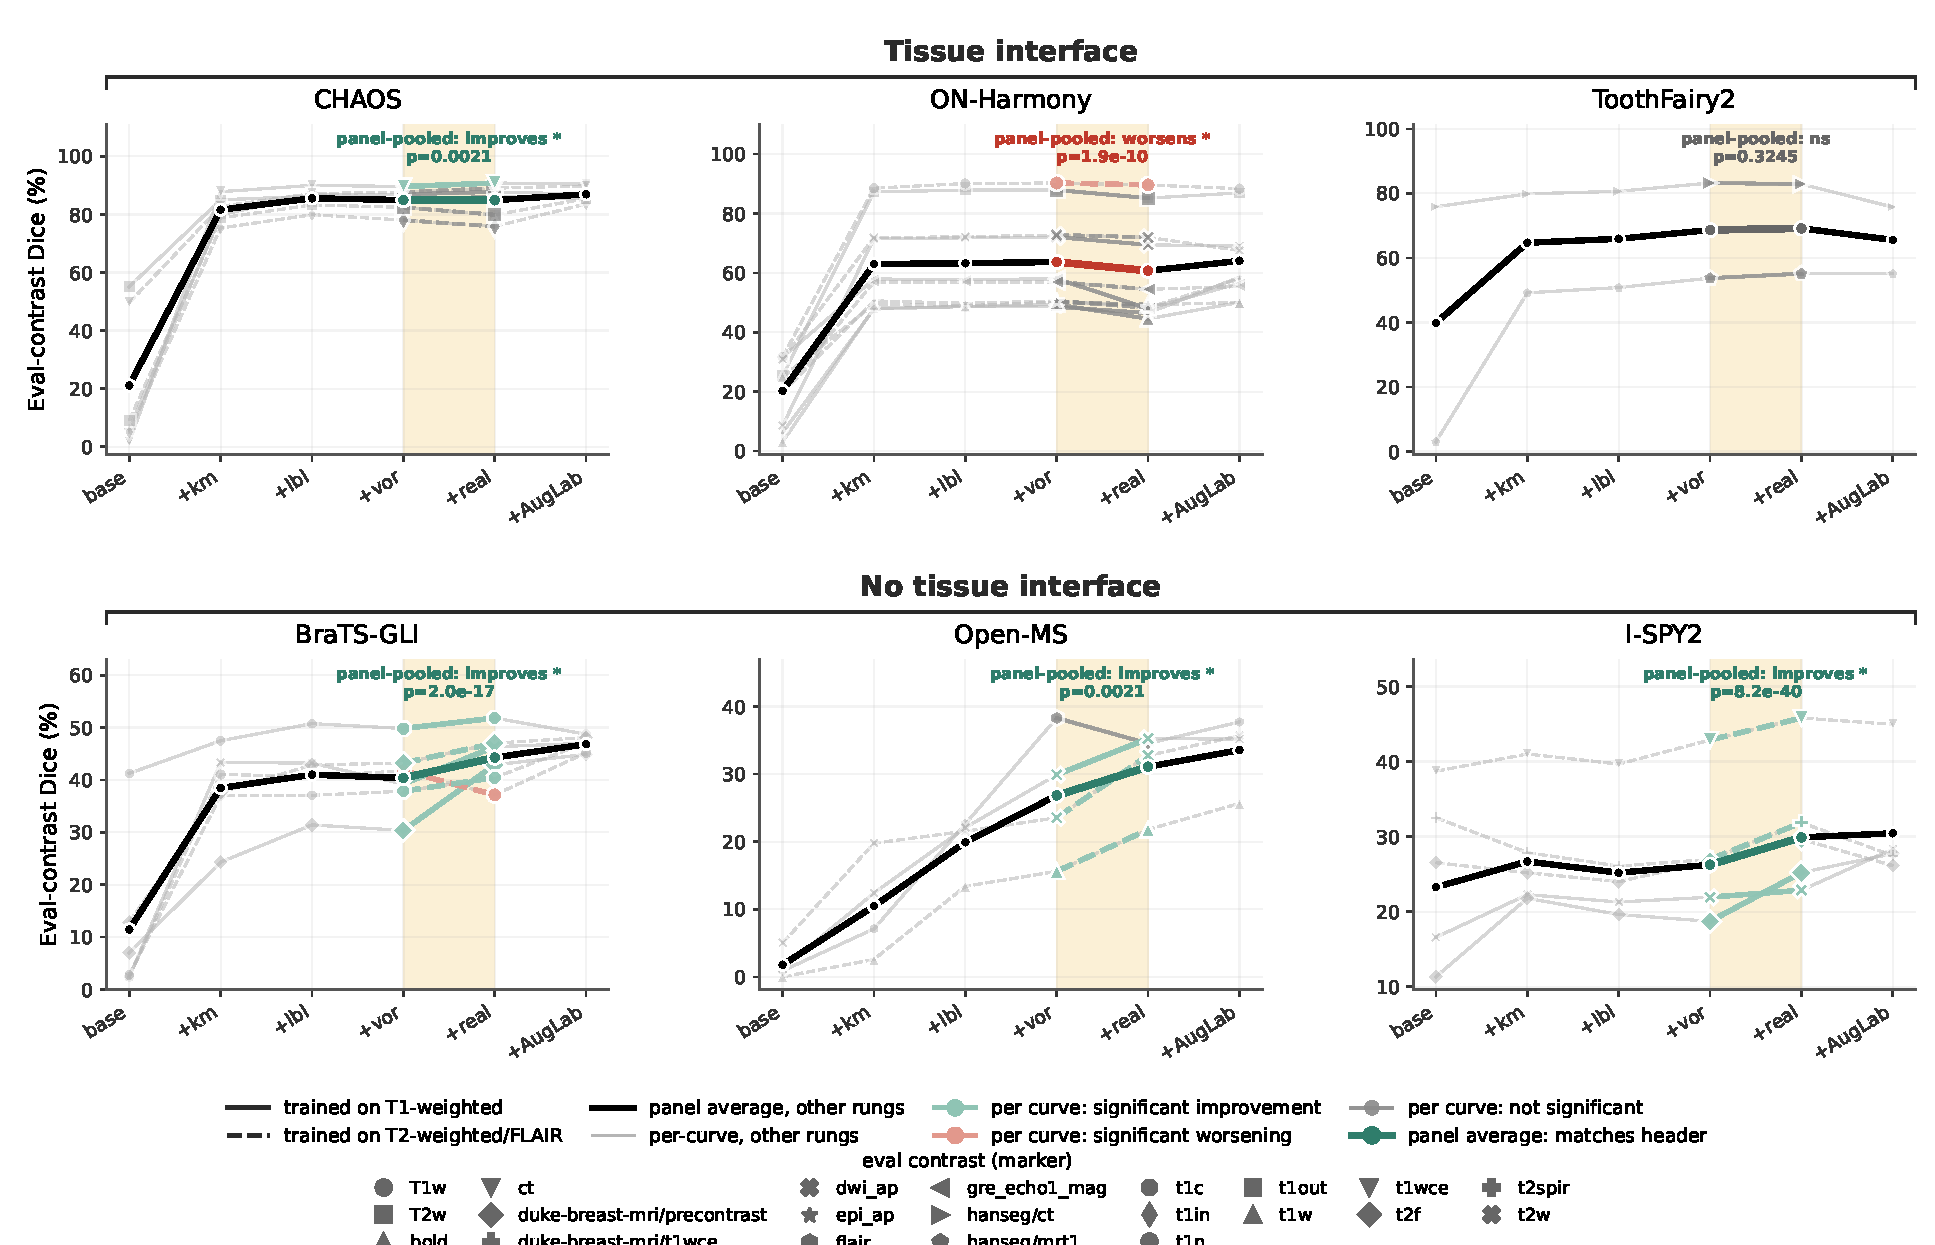
\includegraphics[width=\linewidth]{figures/per_contrast_curves/fill_swap_per_contrast}
\caption{The one-variable test (rung sequence as above), shown per held-out
\emph{eval contrast} rather than pooled, one panel per dataset, grouped by
boundary type. Each thin line is one (training modality, eval contrast)
pair, an external cohort's contrasts included; only its real-fill segment (shaded band) is coloured, by that curve's
\emph{own} significance at this one step (Holm-corrected paired Wilcoxon
within that ladder's own contrast family) -- light teal = significant
improvement, light red = significant worsening, grey = not significant --
since that is the only step being tested; every other segment is plain
grey context. The bold black line is the panel's pooled average across
every curve and training modality, with its own real-fill segment coloured
to match the panel-level annotation above it exactly: a single p-value
pooling \emph{both} training modalities into one paired Wilcoxon test
(Holm-corrected across the six panels) -- a coarser, dataset-level
reading than \cref{tab:dissociation}'s finer per-(task,modality) rows,
which keep the modality-specific breakdown this panel-level view
collapses. Four of the six panels move significantly in the predicted
direction; ToothFairy2's is not significant either way, which is the
prediction for a tissue-interface target coming true rather than a null
result; and ON-Harmony's panel-pooled effect is a significant
\emph{worsening} (labelled accordingly, not a low $p$ defaulting to read
as ``helps''). Solid/dashed = trained on a T1-weighted vs.\ T2-weighted/FLAIR
contrast; marker shape = eval contrast, one mapping reused across every
panel. Dice numbers pooled per ladder in \cref{tab:dissociation}; HD95 in
\cref{sec:suppl-persetting}.}
\label{fig:ladder}
\end{figure*}

\begin{table}[t]
\centering
\small
\setlength{\tabcolsep}{4pt}
\begin{tabular}{llcc}
\toprule
Task & boundary type & $\Delta$ Dice & $p$ \\
\midrule
CHAOS T1in      & tissue interface & $+1.07$ & 8.6e-4 \\
CHAOS T2spir    & tissue interface & $-1.14$ & 0.50 \\
ON-Harmony T1w  & tissue interface$^\dagger$ & $\mathbf{-4.48}$ & 4.6e-6 \\
ON-Harmony T2w  & tissue interface$^\dagger$ & $-1.43$ & 1.4e-7 \\
ToothFairy2 CBCT & tissue interface$^\ddagger$ & $+0.51$ & 0.65 \\
\midrule
Open-MS FLAIR   & no tissue interface & $\mathbf{+7.69}$ & 3.7e-4 \\
Open-MS T1w     & no tissue interface & $+0.79$ & 0.65 \\
Brats-GLI T1n   & no tissue interface & $\mathbf{+7.22}$ & 2.9e-25 \\
Brats-GLI T2w   & no tissue interface & $+0.60$ & 0.50 \\
I-SPY2 T1-CE    & no tissue interface & $+3.72$ & 1.9e-15 \\
I-SPY2 T2w      & no tissue interface & $+3.59$ & 8.7e-25 \\
\bottomrule
\end{tabular}
\caption{Effect of replacing label-style noise fill with the real-intensity
remap, \emph{holding the partition and per-region statistics fixed}, on
out-of-domain Dice, across all six tasks (both training modalities each,
except CBCT-only ToothFairy2). $p$ is a Holm-corrected paired Wilcoxon test
on this one step, pooled over each row's held-out contrasts, corrected
across all eleven rows. The separation is by \emph{magnitude}: every effect
above $+1.1$ Dice is on a no-tissue-interface target, and the tissue-interface
rows span $-4.48$ to $+1.07$ with no gain larger than a point. Within the
no-tissue-interface group the size still varies --- large on Open-MS FLAIR,
Brats-GLI T1n and both I-SPY2 rows, small on Open-MS T1w and Brats-GLI T2w
--- but the sign never flips there. HD95 for this same step is reported in
\cref{sec:suppl-persetting}, where the separation is not as clean.
$^\dagger$31 regions, all bounded by a genuine tissue-type transition
(ventricles against CSF, cortex/nuclei against white matter), just packed
across near-total brain volume rather than a handful of large organs like
CHAOS -- see discussion below.
$^\ddagger$ToothFairy2 acquires CBCT only, so this row's held-out axis is
cross-\emph{dataset} (HaN-Seg CT and MR-T1) rather than a second in-house
contrast; it is the one row whose estimand differs in that respect, and we
mark it rather than pooling it in silently.}
\label{tab:dissociation}
\end{table}

\cref{fig:ladder,tab:dissociation} show the predicted dissociation between
the two kinds of target the ablation was designed to separate: preserving
real texture is worth a large, significant Dice gain on tasks whose targets
are defined by tissue appearance and have no anatomical interface, and
close to nothing -- rarely a significant cost -- on tasks with one. This is
the paper's central result: it identifies \emph{when} texture preservation
matters, and it does so by intervention rather than by correlation across
methods. Mandible is the sharpest test of the prediction because it was
classified before the number was computed: a mandible is a bone with an
unambiguous interface to the soft tissue around it, so the ablation should
do nothing there, and it does nothing ($+0.51$ Dice, $p=0.65$) despite
having the third-largest case pool of any row.

The size of the gain still varies within the no-tissue-interface group: it is
large on Open-MS FLAIR, Brats-GLI T1n and both Breast rows, and much smaller
-- no longer significant on its own -- on Open-MS T1w and Brats-GLI T2w,
though the sign never flips. We read this as the same mechanism at reduced
strength rather than a contradiction of it, and note it rather than paper
over it. One driver is visible in the Breast rows: the effect is largest
where the distribution shift is hardest. Within I-SPY2's own cohort the
T1-CE-trained model gains $+0.93$ Dice at this step, but on the external
Duke cohort's pre-contrast acquisitions the same step is worth $+6.50$. A
reader should therefore expect these numbers to understate the effect on
tasks whose held-out axis stays close to home, not overstate it.

Does ON-Harmony's negative pooled Dice (\cref{tab:dissociation}) reflect the
same tissue-interface pattern as CHAOS, or is it a genuinely different
phenomenon driven by how densely it labels the brain? We checked directly
rather than speculating: ON-Harmony's 31 regions -- the standard
subcortical parcellation (lateral/3rd/4th ventricles, cortex, white matter,
cerebellar white matter and cortex, brainstem, eight deep grey nuclei) --
are, without exception, bounded by a genuine tissue-type transition: CSF
against tissue for the ventricles, grey matter against white matter for
cortex and the nuclei. There is no texture-only, no-interface label in the
set, unlike a tumour or lesion margin. ON-Harmony's result is therefore not
a third pattern requiring its own account; it groups with CHAOS as a
tissue-interface task, just one that labels near-total brain volume rather
than a handful of organs -- plausibly why the effect is larger in magnitude
than CHAOS's near-null one, though still never a significant \emph{gain}.
Whether that labelling \emph{density} carries its own separate effect,
beyond boundary type alone, is a question one densely-labelled task cannot
answer; we leave it to a dedicated follow-up with a second such task.

Two further properties of this test are worth stating explicitly. First, it
is not a comparison between methods but between two versions of the same
method that differ in one component, so it cannot be explained by
differences in augmentation strength, partition granularity or training
schedule. Second, the test is independent of whether PALETTE wins the
task: it is specifically the \emph{texture} ingredient whose effect varies,
while the remaining ingredient, the wider space of region-to-region contrast
relationships, continues to help throughout. Breast makes that independence
concrete in the direction least convenient for us --- the texture step is
strongly positive there while the full recipe places second
(\S\ref{subsec:e-main}) --- and ON-Harmony makes it concrete in the other,
with a negative texture step on a task where PALETTE leads.

\paragraph{Why the margin over Auglab is thin where it is.} The same
gradient-orientation measurement that isolates texture in
\cref{subsec:e-ablation} also explains the size of the remaining gap: Auglab
is \emph{not} a texture-destroying method, retaining a normalized-gradient-field
similarity to the source scan only modestly below PALETTE's and far above
the label-style methods' (\cref{sec:suppl-ngf}). Where the target has no
tissue interface and texture is therefore the operative cue, two methods
that both largely preserve texture should be expected to land close
together --- which is what we observe. The large margins appear against the
methods that discard texture, and the thin ones against the method that
does not.

\paragraph{Supporting analyses.} A component ablation separating the
contributions of the $k$-means partition, the Voronoi sub-parcellation and
the signed remap is given in \cref{sec:suppl-mechanism}. An independent,
segmentation-free measurement of texture fidelity -- gradient-orientation
agreement between each augmented volume and its source -- confirms that
texture is what changes at the fill-swap step and is reported in
\cref{sec:suppl-ngf}. Per-setting tables for all eleven source-modality
settings are in \cref{sec:suppl-persetting}.

